% Komponentendiagramm des Projektes
\section{Komponentendiagramm}

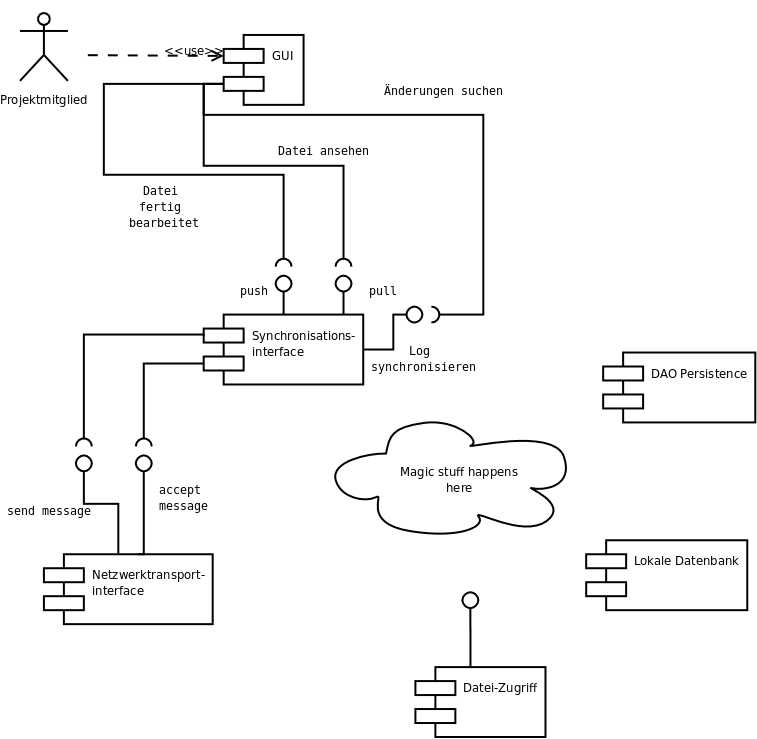
\includegraphics[width=0.98\textwidth]{../../uml/component_diagram.png}

Das Projekt ist in folgende Komponenten aufgeteilt:

% Wie man sieht habe ich sehr viel dazugeschrieben. Allgemein ist mein Verständnis von einer Komponente das, dass ich von ihr wissen will, wofür ich sie nutzen kann und was sie mir für Services anbietet. ~simon

% Es sollen zuerst die Aufgaben jeder Komponente beschrieben.
% Danach kann auf Verbindung zu anderen Komponenten eingegangen werden: Nicht durch Abläufe, es sollen die Beziehungen beschrieben werden
% Die Beziehung ist, dass der Core immer die Kontrolle hat, aber dass er eben auch auf Callbacks/Events von den anderen Komponente wartet
% Nicht die internen Abläufe beschreiben, und bei allen Komponenten auf gleichem Detailniveau bleiben.
% ~johannes



\subsection{Core}
In der Core-Komponente befindet sich die Business Logic der Applikation. Der Core arbeitet hier sozusagen als Übersetzer zwischen den einzelnen Komponenten. So wird zum Beispiel im Core bestimmt, was die Applikation zu tun hat, wenn ein Benutzer in der Grafischen Benutzeroberfläche auf ``Aktualisieren'' drückt oder eine Datei löschen möchte. Da die komplette Logik im Core und nicht in der GUI selbst implementiert wird, ist es technisch leicht möglich, alternative User Interfaces anzubinden, ohne irgendwelche Programmlogik erneut zu programmieren.
Neben dem Bereitstellen der Funktionalität für das User Interface registriert sich der Core auch bei anderen Komponenten als Observer, um auf Ereignisse dieser Komponenten (z.B. das Verändern einer Datei im Dateisystem oder der Empfang einer Netzwerknachricht) reagieren zu können. Was genau beim Eintreffen eines Ereignisses geschieht, wird ausschließlich im Core festgelegt. Hierbei ändert allerdings nicht der Core selbst, z.B. eine Statusbar, vielmehr weist er die GUI Komponente auf Änderungen hin, die für den Benutzer von Interesse sind, oder die seine Aufmerksamkeit/seinen Input benötigen.

\subsection{Graphical User Interface}
Die grafische Benutzeroberfläche, mit der der Endanwender arbeitet, ermöglicht Zugriff auf alle von der ``Core''-Komponente für Endbenutzer zur Verfügung gestellten
Funktionalitäten.

% Persistence NICHT Database Persistence, es ist nicht festgelegt dass wir eine Datenbank verwenden ~simon
\subsection{Persistence}
Die Persistence Komponente abstrahiert den Zugriff auf die Daten, die für den Betrieb gespeichert werden müssen. Diese umschließen nicht die Dateien. Es wird das Konzept des Data Hiding umgesetzt, wodurch erreicht werden kann, dass die anderen Komponenten nur auf definierte Weise die Daten verwenden. Für die Speicherung der Daten kann eine relationale Datenbank verwendet werden.

\subsection{Synchronisation Services}
Die Synchronisationskomponente ist für die Verteilung von Änderungsinformationen und Dateninhalten an andere Projektmitglieder/Clients zuständig. Hierbei werden spezielle Strategien, wie z.B. das Abgleichen von Verzeichnislisten, Hashlisten o.ä. vor den restlichen Komponenten versteckt.

\subsection{File System Services}
Die File System Services kapselt den Zugriff auf Dateien im Dateisystem. Außerdem kann diese Komponente durch entsprechende Strategien feststellen, ob Dateien geändert wurden oder in die Projektordnerstruktur kopiert wurden und dies dem Core mitteilen, welcher wiederum entsprechende Aktionen veranlasst.

\subsection{Interclient Communication Service}
Der Interclient Communication Service kapselt die vollständige Kommunikation zwischen den Clients (über das Netzwerk) und gibt die entsprechenden Nachrichten an den Core weiter. So ist es leicht möglich, verschiedene Netzwerk-backends (z.B. XMPP oder RMI) zu unterstützen, welche für den Core und somit für den Benutzer transparent sind. Außerdem wird die Authentifizierung der Nutzer in dieser Komponente durchgeführt, was es erlaubt, die Anwendung unter anderem an verschiedenste Authentifizierungssysteme anzubinden.

\subsection{Schnittstelle GUI - Core}
Die grafische Benutzeroberfläche greift auf eine Schnittstelle des Core's zu. Diese Schnittstelle stellt alle notwendigen Funktionen zur Verfügung um die Elemente der grafischen Benutzeroberfläche mit Inhalten zu füllen. Außerdem ruft die GUI beim vom Benutzer ausgelösten Events (z.B. das drücken einer Schaltfläche) die Funktion mit der entsprechenden Logik im Core auf.

